\documentclass{article}
\usepackage{graphicx}
\usepackage{xspace}
\usepackage{balance}  
\usepackage{amsmath}  
\usepackage{subcaption}
\usepackage{comment}
\usepackage{tablefootnote}
\usepackage{booktabs}
\usepackage{float}
\usepackage{url}
\usepackage{array}
\usepackage{pbox}
\usepackage{mdwlist}
\usepackage{footnote}
\usepackage{geometry}
\geometry{margin=1in}

\begin{document}
	
\title{Interactive Machine Learning Interface}
\author{Lilong Jiang(jiang.573)}
\date{}
\maketitle

\section{Introduction \& Motivation}
% visual data analysis is popular, business intelligence (tableau)
% motivation: interactive visualization, usability, verfication
Interactive visualization analysis is an important research area in information visualization, databases and human-computer interaction(HCI). Previous works and commercial products (e.g. Tableau~\footnote{http://www.tableau.com/‎}) focus on data analysis area, e.g. how to dynamically filtering datasets~\cite{ahlberg1992dynamic, goldstein1994using}, zooming and panning~\cite{rao1994table}, brushing and linking~\cite{doleisch2002smooth, hauser2002angular}. Recently, more works focus on the machine learning and data mining algorithms~\cite{crotty2015vizdom, wu2013scorpion, packer2013visual, turkay2011interactive}. There several motivations for this trend. Firstly in many cases, there exists parameter tuning stage for machine learning algorithms and whether the point belongs to something (e.g. cluster, outlier) really depends on what metric to use, what threshold is set, etc. Secondly, interactive visualization provides much better usuability than traditional programming method. And non-experts can easily use this interfae. Thirdly, it is often common for users to verify results because of multiple reasons, e.g. overfitting and underfitting. In summary, it is necessary to provide an usable interactive interface allowing users to adjust machine learning algorithms on-line.

\section{Work}
The overall user interface (Figure~\ref{fig:kmeans}, Figure~\ref{fig:regression}, Figure~\ref{fig:svm}) is divided into two parts: the left part shows what kind of machine learning method to run and parameters associated with the algorithm. Also users can choose different dataset and it will show the attributes of current manipulated dataset. The right part shows the visualization of dataset and result. We implement interactive interfaces for three machine learning algorithms in the frontend using javascript, d3~\footnote{https://d3js.org/}, and Tornado~\footnote{http://www.tornadoweb.org/}: K-means~\footnote{https://github.com/emilbayes/kMeans.js} (Figure~\ref{fig:kmeans}), linear regression~\footnote{https://github.com/Tom-Alexander/regression-js}(Figure~\ref{fig:regression}) and support vector machine (SVM)~\footnote{https://github.com/karpathy/svmjs} (Figure~\ref{fig:svm}).  Table~\ref{table:operations} summarizes operations that users can perform with our interface. 
\begin{table}[b]
	\centering
	\begin{tabular}{l l}
		algorithms & operations  \\ \hline \hline
		k-means & \pbox{50cm}{(1) Select initial centers or generate centers randomly \\ (2) Adjust number of clusters on-line \\ (3) Color shows different clusters} \\ \hline \hline
		linear regression & \pbox{20cm}{(1) Adjust function's intercept by moving the line \\ (2) Adjust function's slope and intercept by dragging end points \\ (3) Dynamically show the function and square loss} \\ \hline \hline
		svm & \pbox{20cm}{(1) Select different kernel \\ (2) Select which features to use by dragging into or out space \\ (3) Dynamically show accuracy, precision, recall and confustion matrix}
	\end{tabular}
	\caption{Operations}
	\label{table:operations}
\end{table}

\begin{figure}[h!]
	\centering
	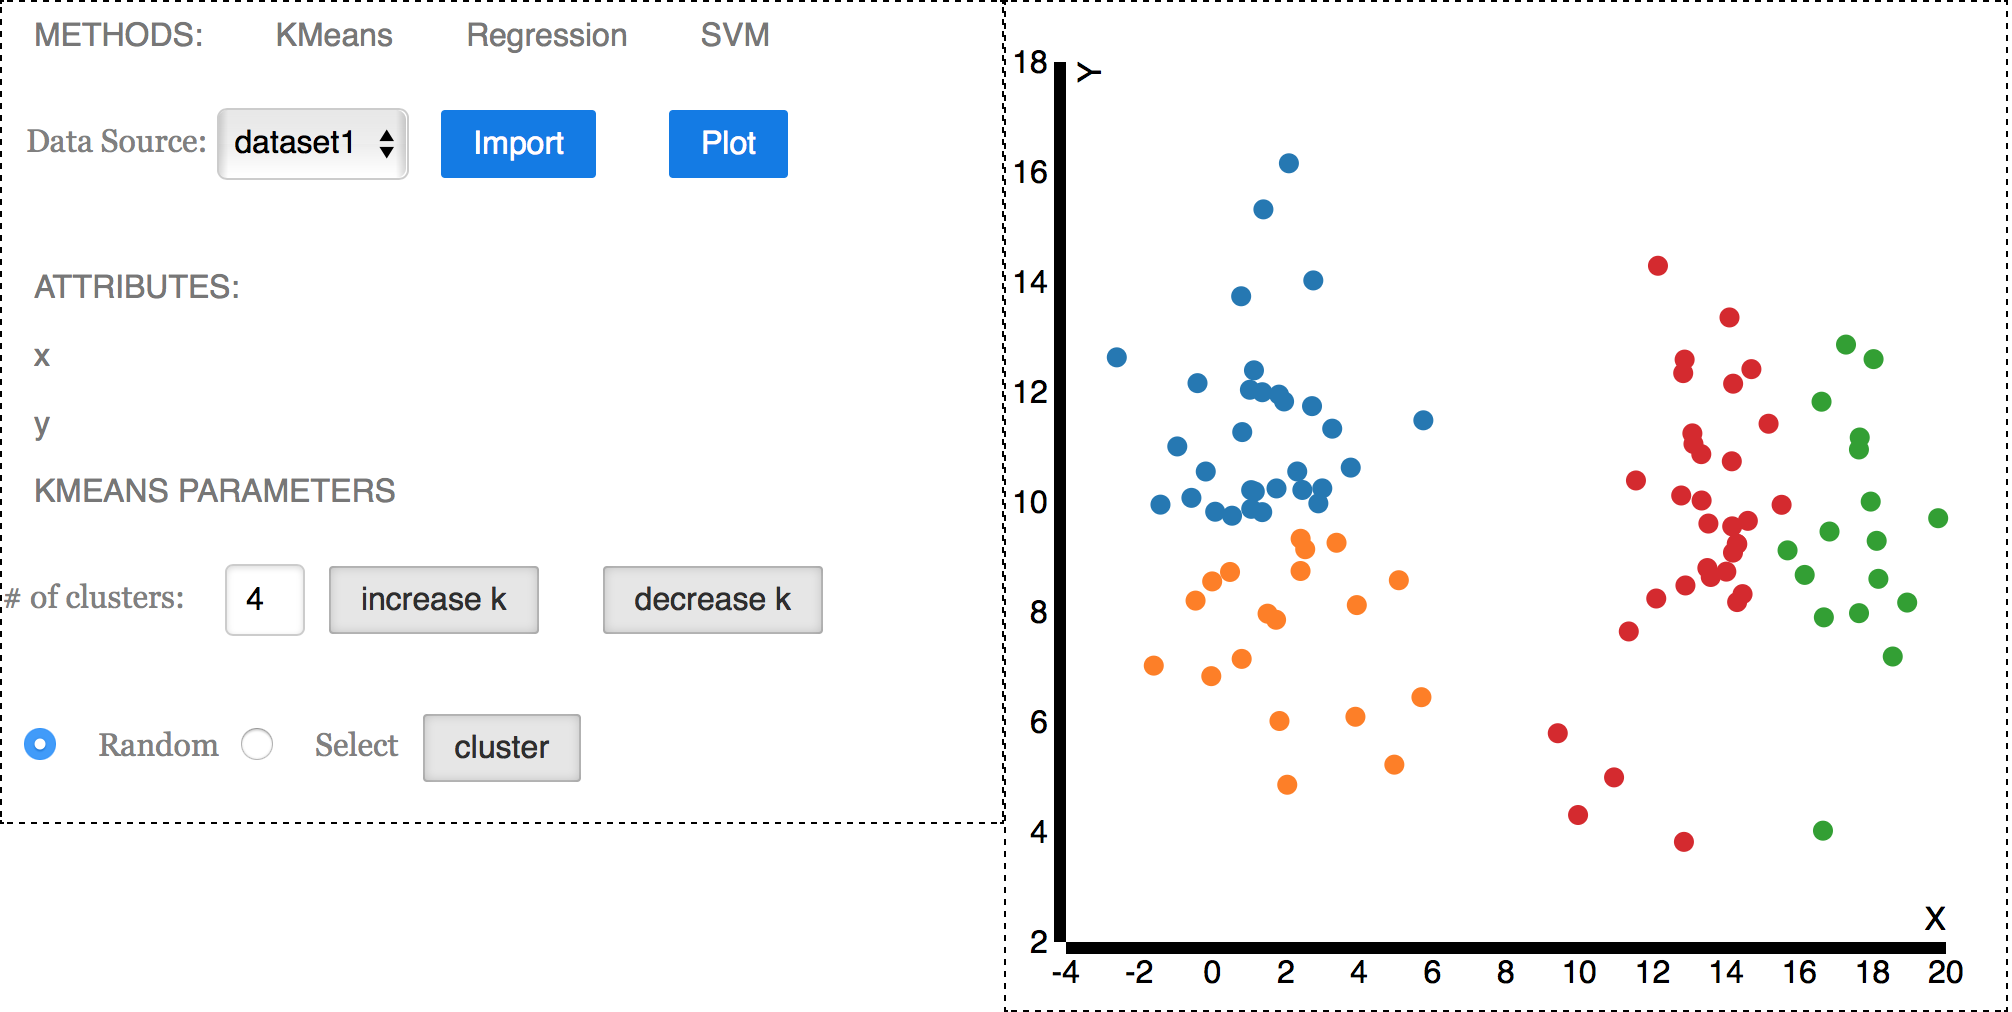
\includegraphics[width=\textwidth]{figs/kmeans}
	\caption{K-means}
	\label{fig:kmeans}
\end{figure}
\begin{figure}[h!]
	\centering
	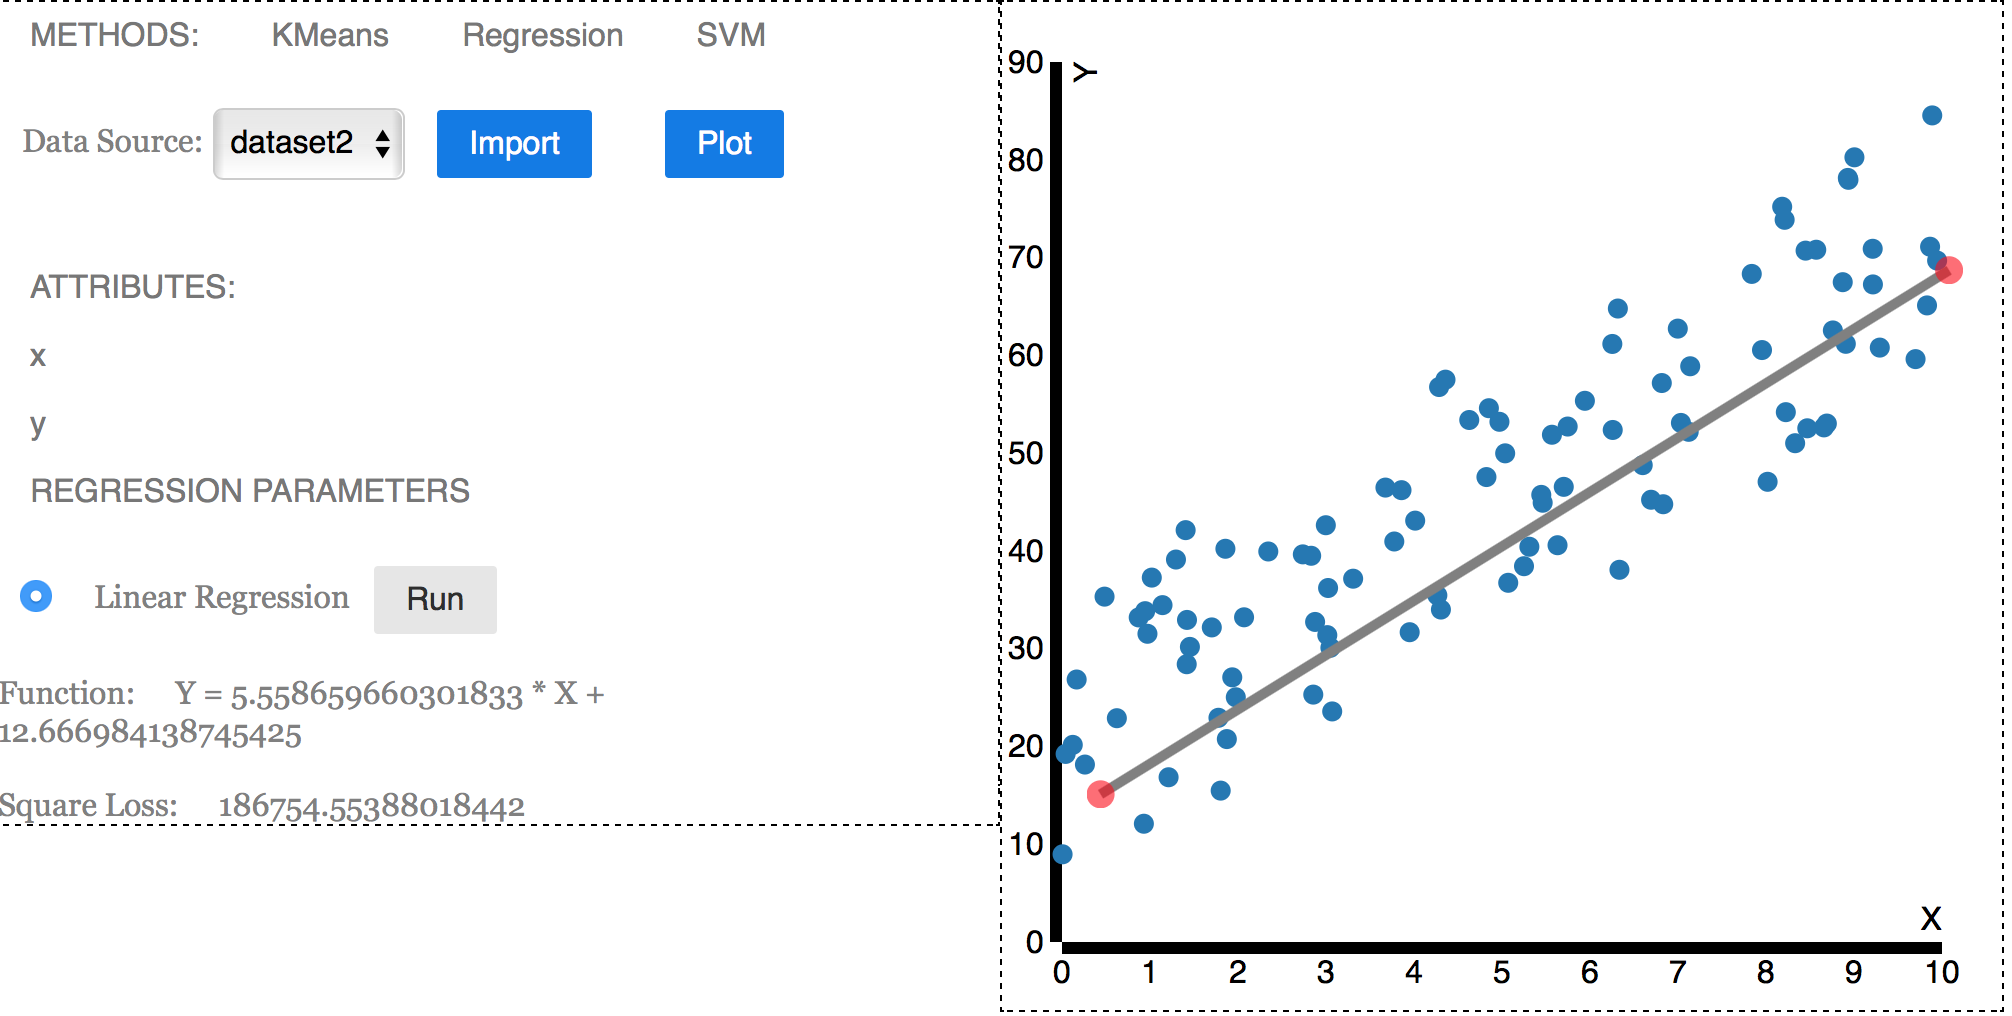
\includegraphics[width=\textwidth]{figs/linearregression}
	\caption{Linear Regression}
	\label{fig:regression}
\end{figure} 
\begin{figure}[h!]
	\centering
	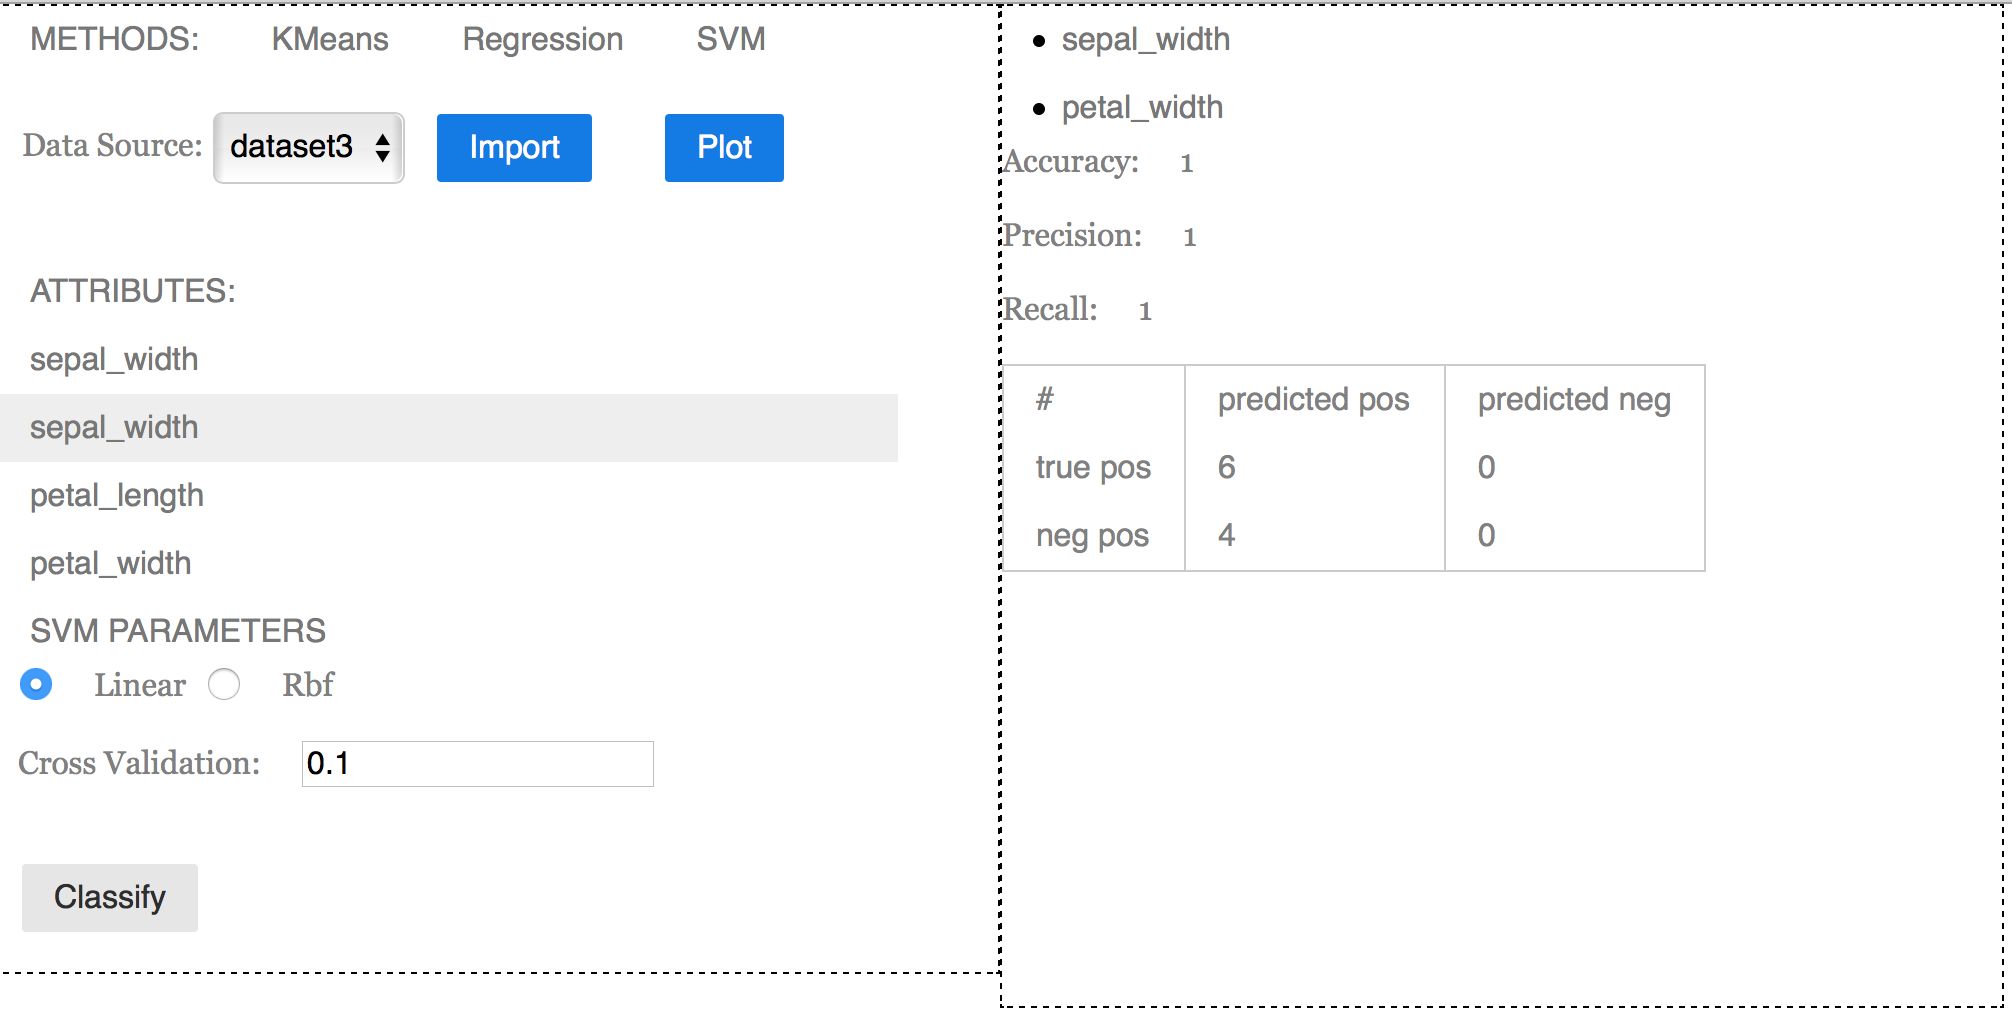
\includegraphics[width=\textwidth]{figs/svm}
	\caption{SVM}
	\label{fig:svm}
\end{figure} 


\section{Performance Experiments}
In this section, we focus on performance experiments since in the interactive environment, it is necessary to keep an interactive performance. \\
\textbf{Computer Configuration:} The experiment is run a MacBook Pro with 2.7 GHz Intel Core i5 and 8G memory.\\
\textbf{Dataset:} For K-means, we sample from 2 bivariant normal distributions and run K-means for 100 interations. For linear regression, we generate dataset from a linear function and add random noise to each point. For SVM, we use Skin Segmentation Data Set from UCI~\cite{skinsegment}.  There are totally 3 numerical attributes and 2 classes. We randomly sample from both classes. \\
\textbf{Results:} For linear regressions, for 2 million number of points, it just takes less than 200ms to calculate the regression function and for each update. It is able to keep an interactive performance. However, for k-means and SVM, it is kind of hard. Figure~\ref{fig:kmeans_performance} and Figure~\ref{fig:svm_performance} show that the running time can easily be greater than 1 second for both k-means and SVM. Optimization is necessary for both algorithms to maintain an interactive performance. \\

\begin{figure*}[t!]
	\centering
	\begin{subfigure}{0.47\textwidth}
		\centering
		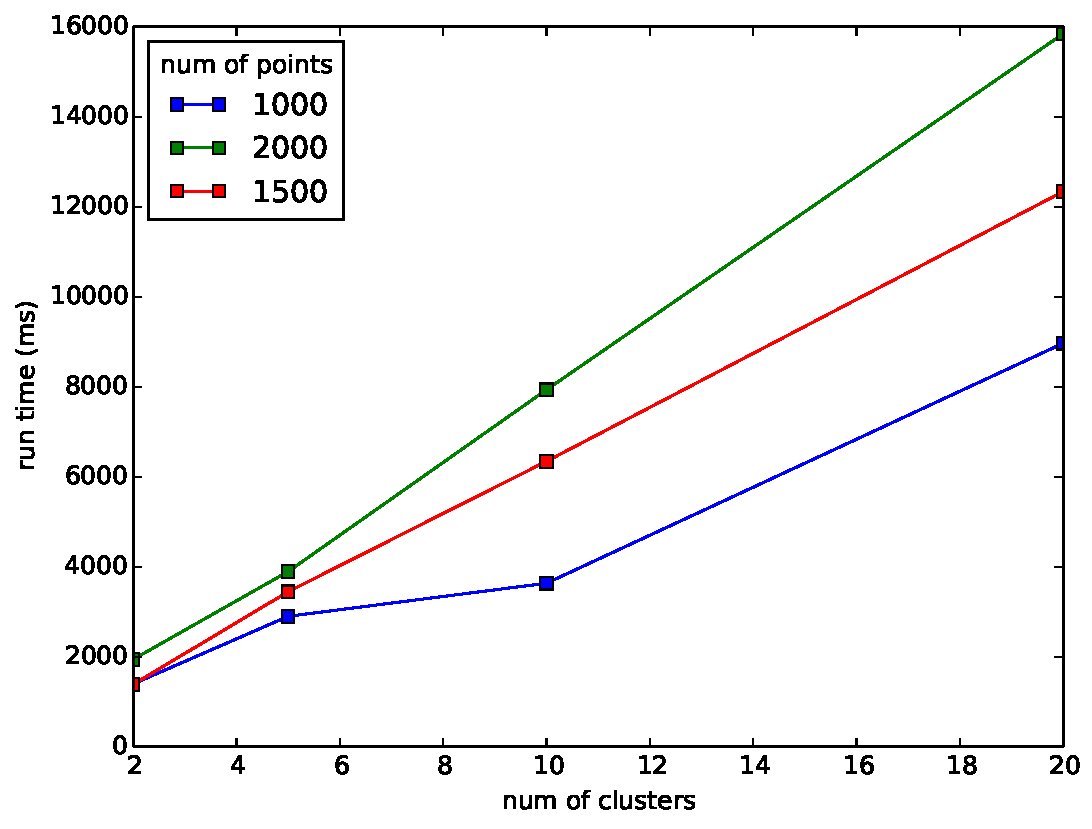
\includegraphics[height=5cm]{figs/kmeans_result}
		\caption{K-means performance}
		\label{fig:kmeans_performance}
	\end{subfigure}%
	\begin{subfigure}{0.47\textwidth}
		\centering
		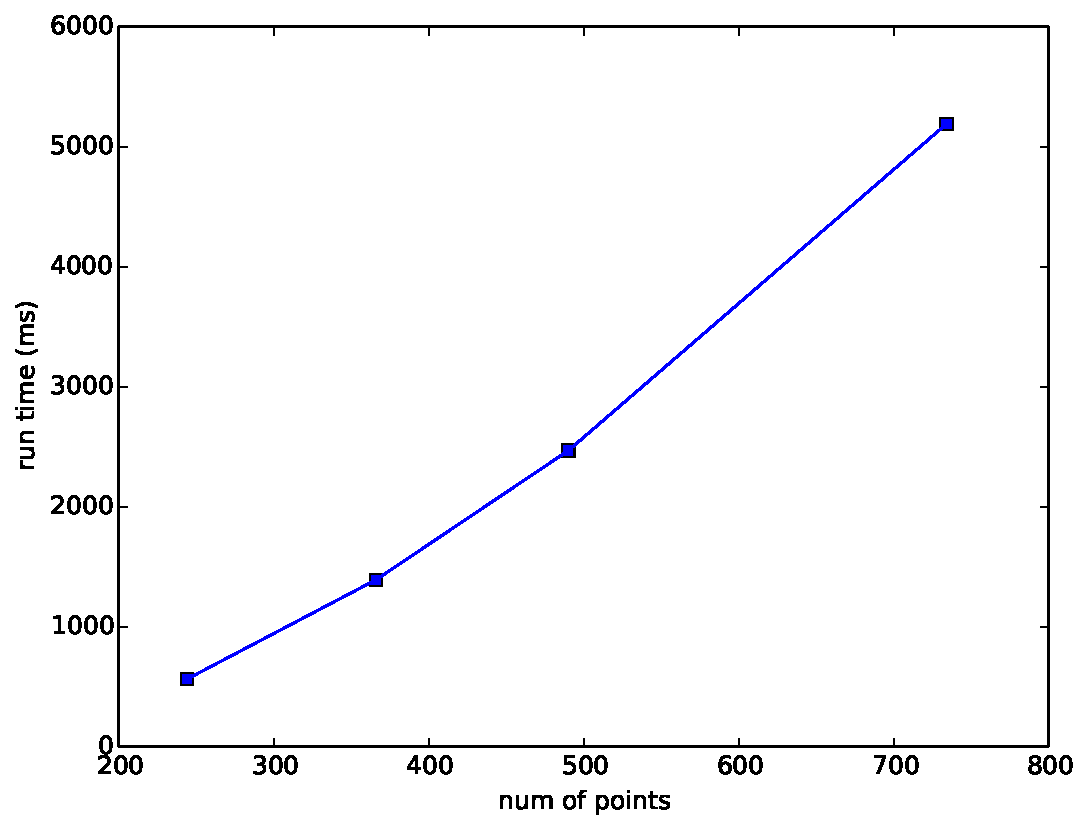
\includegraphics[height=5cm]{figs/svm_result}
		\caption{SVM performance}
		\label{fig:svm_performance}
	\end{subfigure}
	\caption{Performance}
\end{figure*}

\section{Limitations \& Conclusions \& Future Work}
In this project, we focus on usability point. There are several limitations for this project. The first is interactive performance when the number of points is large. One method is to run machine learning algorithm in the backend and once it is done, then send it to frontend.  However, users need to pay the internet cost.  Another method is to use an incremental method, which update results incrementally as more data is processed. Works including~\cite{crotty2015vizdom, fisher2012trust} adopts this method. \\
The second is to visualize high-dimensional dataset, and this can be achieved by projection, which is a technique that maps high-dimensional dataset into a small set of dimensions. There are many methods for projection. Some works use dimension reduction, that create latent dimensions that summarize dataset. For example, Principal Component Analysis (PCA)~\cite{jolliffe2002principal}, Multidimensional Scaling (MDS)~\cite{mead1992review}. This method can reveal hidden variables. However, the generated dimensions are usually less intuitive to users. Another method is called feature selection, which selects subset of features to explore. Interactive feature selection is often used to identify relationship between features~\cite{guo2003coordinating, yang2004value} and aid user remove redundant features and choose appropriate features. All these methods can be easily incorporated into our project.  \\
In conclusion, we build an interactive machine learning interface which allows users to visualize dataset, run different kind of machine leanring algorithms, and compare results. Incorporating high-dimensional visualizations, expanding linear regression into other kind of regression types, and allowing supporting large datasets are ideal future work.

\small
\bibliography{main}
\bibliographystyle{plain}
\end{document}